\begin{figure*}[!htb] % concept
  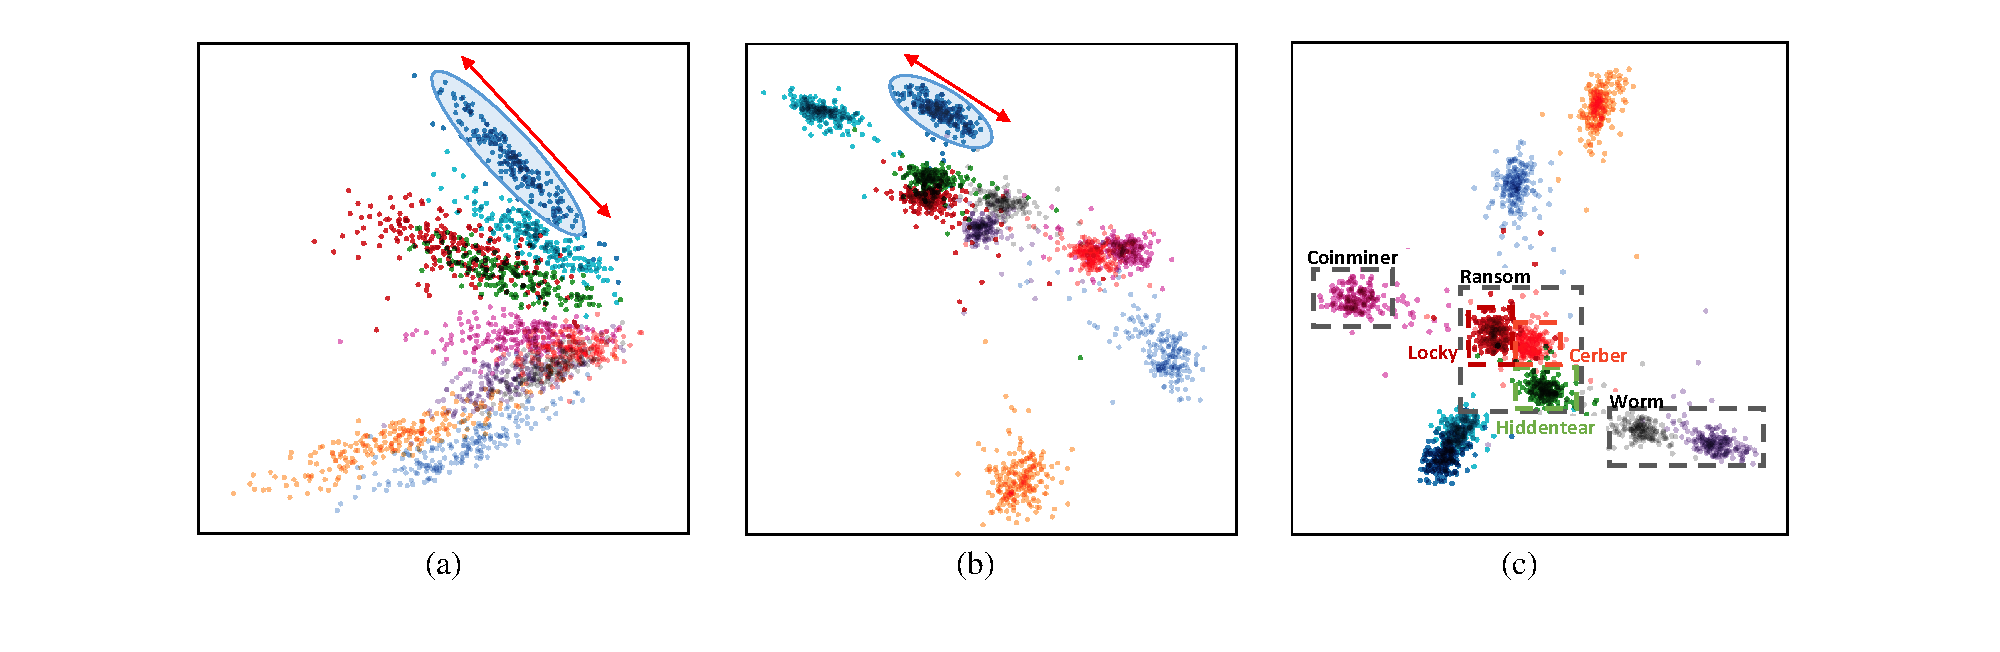
\includegraphics[width=\textwidth]{../../figures/concept_fix.pdf}
  \caption{The concept of our proposed method. Figure (a) shows PCA plot of representation vectors which are trained by single-label classificaion task. Figure (b) shows the vectors trained by training single-label classification task with centerloss. We observe that of center figure's intra-class variance model is smaller than left figure's.
  Figure (c) shows the vectors which are trained by multi-label classification task with multi-label centerloss. It shows that representation vectors whose semantics are simliar are nearly located then others. 
%  
%  왼쪽 그림은 그냥 싱글레이블 클래시피케이션 태스크를 학습해서 얻은 리프레젠 테이션 벡터의 PCA plot이다.
%  	가운데 그림은 싱글레이블 클래시피케이션 태스크를 센터로스를 적용하여 학습해서 얻은 리프레젠테이션 벡터의 PCA plot 이다. 왼쪽 그림에 비해서 intra class variance 가 줄어들었을을 그림에서 확인할 수 있다. 오른쪽 그림은 multilabe 클래싶피케이션 테스크를 센터로스를 적용해서 학습해서 얻은 리퍼르제네테이션 벡터의 Pca plot이다. 왼쪽과 가운데 그림에 비하여 semantically similar sample의 벡터들이 가깝게 위치하였음을 확인할 수 있다. 
  }
  \label{fig:concept}
\end{figure*}

\section{Semantics Aware Representation Learning}
This section describes how the vectore space in which malware is embedded approximates the semantic space. First, we describe malware semantic space and we propose a loss function for training semantic-aware malware representation vectors.

\subsection{Semantic Space for Malwares}

\textbf{The meaning of approximate semantic space of malwares. }
We now take an example of language, thinking of the meaning of certain words. We consider the relationship of those meanings. We can assume that city names and words related to machine learning are located far away from each other. We can also imagine that the words will be near. The similarity of the relationships between words can thus be considered. The relationship between \texttt{King} and \texttt{Queen} is similar to the relationship between \texttt{Man} and \texttt{Woman}. To describe the meanings of these words, we represent them as vectors on a vector space. If the meaning is similar, the distance between the vectors is near. If the meaning is disparate, the distance between the vectors is far away. We also approximate the semantic relationship between words by using operations defined in the vector space, such as \texttt{king - queen = man - woman}.

Similarly, we can imagine the semantic meaning of malicious code. We consider malware as a combination of malicious components. We use the concept of basis and linear combination to describe it as a vector space operation. In other words, we can approximate the semantic space by training the semantic vector of malware to be represented as a linear combination of the semantic component vector.


\textbf{Approximated semantic space. }
Let $X = \{x_1, …, x_n, …, x_N\}$ be a set of malwares.
Let $S$ be a subset of vector space $V$ of dimension $d$ and let semantic component set $S = \{s_1, ... , s_k, … s_K\}$ be a linearly independent subset of $V$.  
Then for every $\mathbf{e} \in E$, there is a linear combination of the sementic component vectors that equals $e$.
\[
\mathbf{e} = c_1\mathbf{s_1} + c_2\mathbf{s_2} + … + c_k\mathbf{s_k} 
\]

where $c_i$ is the i-th element of coefficient vector $ \mathbf{c} = \{c_1, ... , c_k\}$ and we call it as importance coefficents.
We call vector $\mathbf{e}$ as a semantic vector of malware $x$ and there is a nonlinear mapping from $X$ to $E$. 

\textbf{Metric function. }
We use an Euclidean Distance $d(\mathbf{e_i}, \mathbf{e_j})$ for a metric of a set E and it means the function that defines a distance between  semantics of two malwares. 


\textbf{Evidences. } 
If we approximate the semantic space well, then the following querying tasks should work correctly. First, we should be able to retrieve semantically similar malwares by querying malware samples. Second, it should be possible to retrieve by only a combination of semantic components. For example, we should be able to retrieve malwares with these three attributes: \texttt{ransom}, \texttt{downloader}, and \texttt{agent}. Finally, we should be able to retrieve related samples by querying a combination of samples and semantic components such as a sample with attributes \texttt{ransom} and \texttt{downloader} combined with semantic component \texttt{agent}.


\subsection{Solution Overview}
\begin{figure*}[!htb] % qualitative_all
  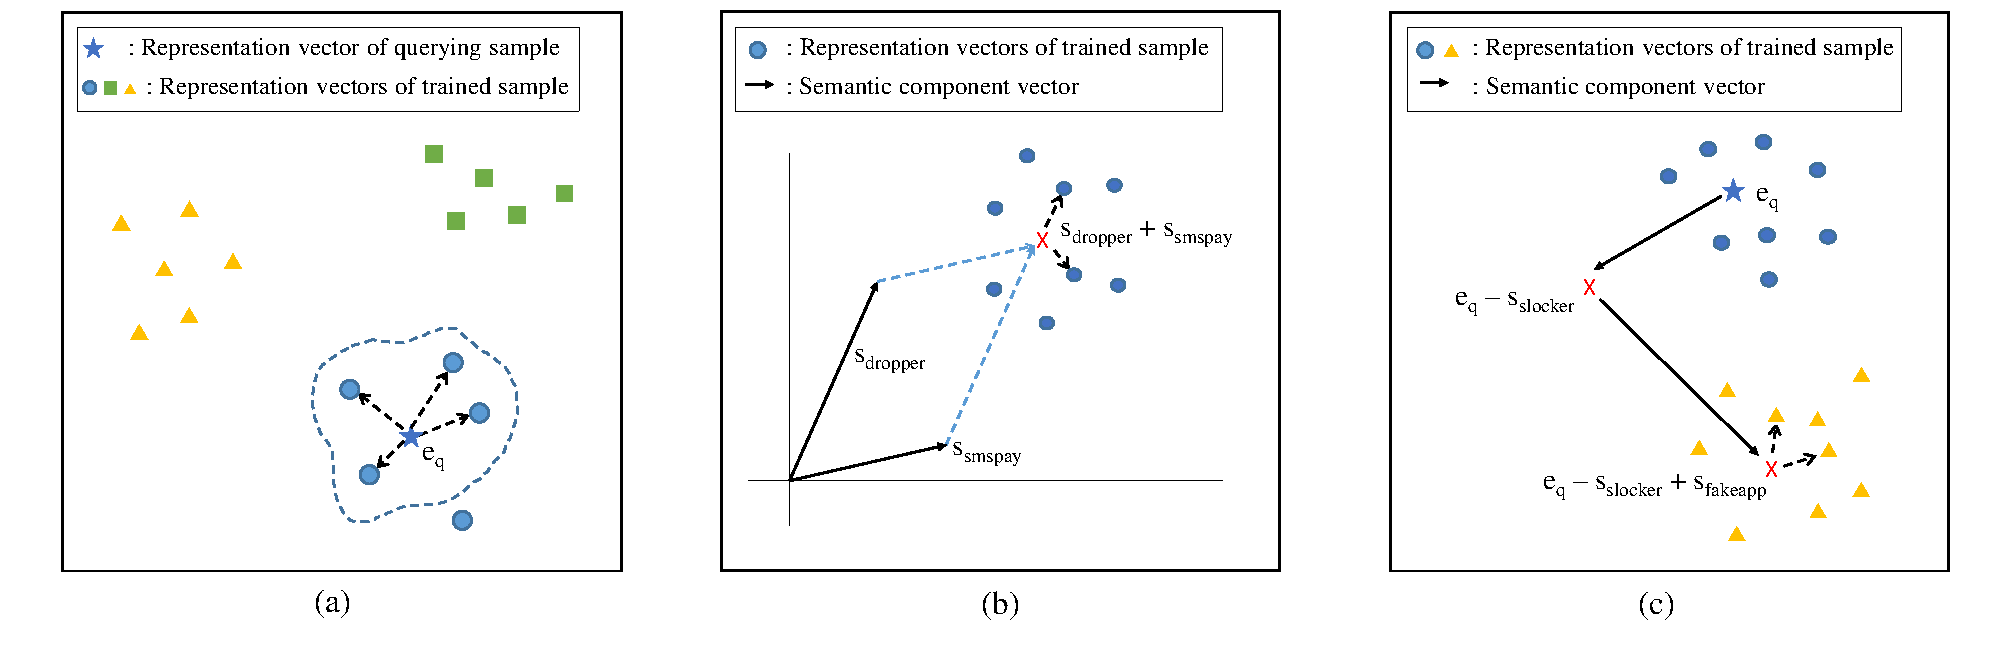
\includegraphics[width=\textwidth]{../../figures/qualitative_all_fix2.pdf}
  \caption{Our malware retrieval system was queried in three ways: malware samples (a), semantic components (b) and a combination of malware samples and semantic components (c).}
  \label{fig:qualitative_all}
\end{figure*}

\textbf{Multi-label classification. }
To train the vector representation, $E$, that reflects the meaning of the malware sample, multi-label classification learning was selected as the auxiliary task. To train this classification task, the neural embedder, $h$, places the representation vectors so that they can be classified by the linear classifier. Most studies that train malware classifiers learn classifiers to classify malware under single label.

However, if you identify a label in a malware domain and create a malware IR system based on it, then the trained embedding vector is insufficient to include the meaning of the sample. Typically, the process of labeling malware is irrational in expressing the meaning of malware. Malware often displays multiple malicious behaviors at the same time. However, existing malware labeling systems do not reflect these attributes. Additionally, naming rules are often globally inconsistent, and even locally, analysts name via differing criteria. Regarding non-prevalent malware, when one labels malware, a name is provided unrelated to the malware’s behavior. These labeling processes prevent the machine learning model from learning the appropriate meanings. 

We use the auxiliary task to classify the labels into multiple labels, and we use vector representations from the auxiliary task to enable retrieval of malware samples of similar meanings.

\textbf{Centerloss. }
To allow the representation vectors of malwares to exist on the semantic space while training multi-label classification in the above way, we use multi-label centerloss. Once in the background, the effect of centerloss is lowering the intra-class variance. This causes centerloss to prevent the intra-class variance from becoming too large and the distance between two samples in the same class to be greater than the distance between two samples of different classes, resulting in improved IR results.

Second, we can locate representation vectors to approximate the semantic space. In the paper proposing a single label centerloss, the template vector is stored in the external memory for each label, and the mean square error (MSE) is set so that the distance between the template vector and the representation vector of sample becomes small. As a result, the representation vector of the sample and the template vector of the class are approximated. Likewise, we store vectors for each semantic component in external memory, and we set the MSE error to a loss function so that representation vector is a linear combination of semantic component vectors.



%그리고, 보틀넥과 시멘틱 컴포넌트들의 합의 차이에 alpha/the number of answer labels 만큼의 곱을 하여 각 레이블을 업데이트해준다. 알파는 하이퍼파라미터로, 템플릿 벡터와 보틀넥을 얼마나 섞어서 기존 템플릿벡터를 업데이트할지를 결정해주는 값이다. 

\textbf{Learn to rank. }
In malware labels, there are important labels and those that are not. Considering this importance in creating a MR system is one of the important factors to satisfy the semantic understanding property. For example, in PE format labels, ranking more than labels such as ransom and coinminer rather than agent or downloader would be considered as a semantics-aware search system. To solve this problem, we use weighted centerloss which reflects the importance of labels with constraint. The constraint determines the norm of the semantic components. Euclidean distance, the metric function that we use in retrieval, is affected by the norm of the two vectors when computing distances. The distance between semantic component vector, having a large norm and another component vector is likely to be larger than the distance between component vectors having a small norm. Therefore, in the MR system ranking with Euclidean distance, when malware having a semantic component with a high importance is queried, the malware samples, including the semantic component, are more likely to be searched. This can be regarded as a scoring technique (i.e., tf-idf \cite{baeza1999modern}), making it possible to search documents with specific properties more easily in the existing information retrieval system.
 

\subsection{Proposed Objective Functions}
We propose a new objective function to learn the semantic space by the methods described in the Section 4.2.

\textbf{Multi-label centerloss (MCL). }
The expression of the constrained optimization problem we want to solve is equal to Eq.\ref{eqn:optimization}. This adds a constraint that the distance between the target semantic vector and the representation vector should be less than $\epsilon$ on the negative log likelihood optimization problem, which is the basis of the cross-entropy loss.



\begin{equation}
\label{eqn:optimization}
\min_{\theta, W, \mathbf{b}} J(\theta, W, \mathbf{b}) = -\sum_i{ \sum_j{ y_{mij} \log{\hat{y_{ij}}}}}
\end{equation}

s.t.
\[
h(v_i;\theta) - \mathbf{s}_\text{target} < \epsilon ,
\]
%\[
%||c_i||_2 = cc_i
%\]
for $i \in \{1,2, ..., N\}$ where $\epsilon \geq 0$ and $s_\text{target}$ is a target semantic vetcor.

To find the parameters satisfying the above equation, the final loss function was constructed by adding cross-entropy loss and multi-label centerloss at a ratio of 1:$\lambda$ \cite{wen2016discriminative}. We can formulate the loss function we propose as Eq.\ref{eqn:centerloss}. 

\begin{equation}
\label{eqn:centerloss}
\begin{aligned}
L &= L_s + \lambda L_c \\
 &= -\frac{1}{N}\sum_i{\sum_j{ y_{mij} \log{\hat{y_{ij}}}}} 
+ \lambda \frac{1}{N} \sum_i{( \mathbf{s}_{\text{target}} - h(v_i;\theta))^2}\\
\end{aligned}
\end{equation}

where 
\[
\hat{y_{ij}} = \frac{\exp(Wh(v_i;\theta)+\mathbf{b})}{ 1 + \exp(Wh(v_i;\theta)+\mathbf{b})}
\]

%$L_c = \sum_i^N{||e_i - s_\text{target}||^2}$

  
\textbf{Weighted multi-label centerloss (WMCL). }
As described above, we apply importance coefficients for each semantic component to apply the learn to rank technique to our Malware Information Retrieval System. We added a constraint such that the importance coefficient value is equal to the norm of the semantic component vector. 

\[
||\mathbf{s_i}|| = c_i \text{ for all i }\in \{i = 1,2, ..., M\}
\]

The cross-entropy loss updates the parameters of $ \theta, W, \mathbf{b} $ to improve the accuracy of multi-label classification. Multi-label centerloss updates parameters as follows. First, the parameters of $\theta, W, \mathbf{b} $ are updated so that the embedding vector is close to $\mathbf{s}_{\text{target}} $ via back propagation. Second, the semantic components are updated so that $ \mathbf{s}_{\text{target}} $ is close to the representation vector. When updating, we divide difference vector between $\mathbf{s}_{\text{target}}$ of current step and representation vector equally and we add it to each semantic component vectors, such that $\mathbf{s}_{\text{target}}$ of next step to be locate at Internally dividing point of current $\mathbf{s}_{\text{target}}$ and representation vector of sample. 

There are several methods to combine semantic component vectors, we propose summation model and average model. The performance of each model can be found in Section 5.

The process of parameters and semantic component update can be found in Figure.\ref{fig:update} and Algorithm.\ref{alg:centerloss}

%average model 은 semantic component 가 추가되거나 제거될 때 embedding vector 의 변화가 많이 필요하지 않다는 장점이 있다. 어떤 semantic component 를 갖고 있는지 모르는 Sample 과 semantic component 의 조합으로 쿼링하는 태스크를 수행하기 어렵다는 단점이 있다. 

\begin{figure}[!htb] % update
  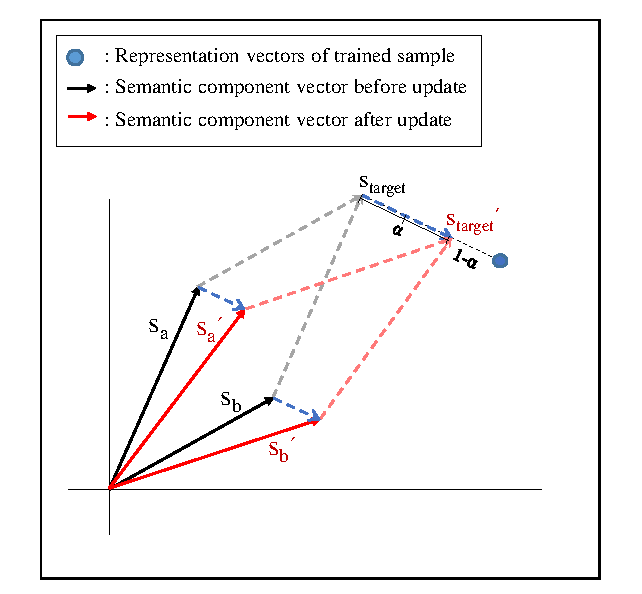
\includegraphics[width=\columnwidth]{../../figures/update.pdf}
  \caption{The semantic components are updated so that $ \mathbf{s}_{\text{target}} $ is close to the representation vector. When updating, we divide difference vector between $\mathbf{s}_{\text{target}}$ of current step and representation vector equally and we add it to each semantic component vectors. Thus $\mathbf{s}_{\text{target}}$ of next step is located at internally dividing point of current $\mathbf{s}_{\text{target}}$ and representation vector of sample. 
}
  \label{fig:update}
\end{figure}


\begin{algorithm}[!htb]%centerloss
\SetAlgoNoLine
\DontPrintSemicolon

\SetKwFunction{Ftarget}{getTargetSemanticVectors}
\SetKwFunction{Fnew}{getNewSemanticComponentVectors}

\KwIn{Extracted handcrafted features of training data $v_i$ and their semantic components $\mathbf{y}_i$. Initialized parameters $\theta$ in neural embedder. parameters $W, \mathbf{b}$ in classifier. initialized semantic component vectors $S$.Importance coefficients $\textbf{c}$. Hyperparameter $\lambda$, $\alpha$, learning rate $\mu$. The number of semantic compoenents $K$}
\KwOut{The parameters $\theta$, $W$, $\mathbf{b}$ }
\Repeat{converge}{
    $\mathbf{s}_\text{target} = \Ftarget(\mathbf{s}_{\mathbf{y}})$ \\
	Compute total loss by $L = L_s + \lambda L_c$\\
	Update parameters $\theta$ by $\theta \leftarrow \theta - \mu \frac{\partial L}{\partial\theta}$ \\
	Update parameters $W$ by $W \leftarrow W - \mu \frac{\partial L}{\partial W}$\\
	Update parameters $\mathbf{b}$ by $\mathbf{b} \leftarrow \mathbf{b} - \mu \frac{\partial L}{\partial \mathbf{b}}$\\	
	Update semantic component vectors $S$ by $S \leftarrow \Fnew(S, \mathbf{s}_{\text{target}}, \mathbf{e}, \alpha, \mathbf{c})$
	
	}
  
  \;  
  \SetKwProg{Fn}{Function}{:}{}
  \Fn{\Ftarget{$\mathbf{s}$}}{
    $M \leftarrow $ The number of semantic components \\
  	
    
	\If{Summation Model}
	{$\mathbf{s}_{\text{target}} \leftarrow \sum_i^M{s_i}$}
	\ElseIf{Average Model}
	{$\mathbf{s}_{\text{target}} \leftarrow \frac{1}{M}\sum_i^M{s_i}$}    
    
    \KwRet $s_{\text{target}}$\;
  }
  \;
    
  \SetKwProg{Pn}{Function}{:}{}
  \Pn{\Fnew{$\mathbf{s}$, $\mathbf{s}_{\text{target}}$, $\mathbf{e}$, $\alpha$, $\mathbf{c}$}}{
    $M \leftarrow $ The number of semantic components \\
    \ForEach{$i \in \{1, 2, ..., K\}$}{
	  \If{Summation Model}
	  {$\mathbf{s}_i \leftarrow \mathbf{s}_i - \frac{\alpha}{M}(\mathbf{s}_{\text{target}} - \mathbf{e})$}
	  \ElseIf{Average Model}
	  {$\mathbf{s}_i \leftarrow \mathbf{s}_i - \alpha (\mathbf{s}_{\text{target}} - \mathbf{e})$ }
	  \If{Weighted Model}
	  {$\mathbf{s}_i \leftarrow \frac{\mathbf{s}_i}{||\mathbf{s}_i||} c_i$}    
    }
    \KwRet $S$
  }
	\caption{The semantics-aware representation vector learning algorithm. }
\label{alg:centerloss}
\end{algorithm}




%
%\begin{algorithm}[!htb]%functions
%  \SetAlgoNoLine
%  \DontPrintSemicolon
%  \SetKwFunction{Ftarget}{getTargetSemanticVectors}
%  \SetKwFunction{Fnew}{getNewSemanticComponentVectors}
%  
%  \SetKwProg{Fn}{Function}{:}{}
%  \Fn{\Ftarget{$\mathbf{s}$}}{
%    $M \leftarrow $ The number of semantic components \\
%  	
%    
%	\If{Summation Model}
%	{$s_{\text{target}} \leftarrow \sum_i^M{s_i}$}
%	\ElseIf{Average Model}
%	{$s_{\text{target}} \leftarrow \frac{1}{M}\sum_i^M{s_i}$}    
%    
%    \KwRet $s_{\text{target}}$\;
%  }
%  \;
%    
%  \SetKwProg{Pn}{Function}{:}{}
%  \Pn{\Fnew{$\mathbf{s}$, $s_{\text{target}}$, $\mathbf{e}$, $\alpha$, $\mathbf{c}$}}{
%    $M \leftarrow $ The number of semantic components \\
%    \ForEach{$i \in \{1, 2, ..., C\}$}{
%	  \If{Summation Model}
%	  {$\mathbf{s}_i \leftarrow \mathbf{s}_i - \frac{\alpha}{M}(s_{\text{target}} - e)$}
%	  \ElseIf{Average Model}
%	  {$\mathbf{s}_i \leftarrow \mathbf{s}_i - \alpha (s_{\text{target}} - e)$ }
%	  \If{Weighted Model}
%	  {$\mathbf{s}_i \leftarrow \frac{\mathbf{s}_i}{||\mathbf{s}_i||} c_i$}    
%    }
%    \KwRet $S$
%  }
%  \;  
%
%  \caption{Definitions of functions. }
%\label{func:functions}
%\end{algorithm}
